% Slides — Capítulo 9: Boletins Meteorológicos e Análise de Cartas
\documentclass[aspectratio=169,11pt]{beamer}
\usepackage{../comum/temameteo}
\graphicspath{{../figuras/cap09/}}

\title[Cap. 9 --- Boletins e Cartas]{Capítulo 9 --- Boletins
Meteorológicos e Análise de Cartas}
\subtitle{Meteorologia Prática}
\author{}
\date{}

\begin{document}

\begin{frame}
  \titlepage
  \vfill
  \atribuicao
\end{frame}

\begin{frame}{Roteiro}
  \tableofcontents
\end{frame}

% ---------------------------------------------------------------
\section{A rede mundial de observação}

\begin{frame}{Tudo começa numa carta idealizada}
  \begin{columns}
    \column{0.4\textwidth}
    \begin{itemize}
      \item Altas, baixas, frentes e o vento contornando — o
            \alert{vocabulário} da previsão sinótica.
      \item Hoje: como se constrói este desenho a partir de milhares
            de observações.
      \item Por que o vento gira assim: Cap.~10.
    \end{itemize}
    \column{0.6\textwidth}
    \figlivroslide{fig_09_1.jpg}{0.54\textheight}{Fig.~9.1 --- carta
      sinótica idealizada: centros, frentes e escoamento}
  \end{columns}
\end{frame}

\begin{frame}{Quem observa o planeta}
  \begin{columns}
    \column{0.4\textwidth}
    \begin{itemize}
      \item Estações de superfície, navios e boias, radiossondas,
            aviões comerciais, satélites (Cap.~8).
      \item Tudo em UTC, 4$\times$/dia (00/06/12/18) — Cap.~1.
      \item Buracos de dados (oceanos, polos): onde a previsão erra
            mais (Cap.~20).
    \end{itemize}
    \column{0.6\textwidth}
    \figlivroslide{fig_09_2.jpg}{0.5\textheight}{Fig.~9.2 --- a rede de
      estações de superfície}
  \end{columns}
\end{frame}

% ---------------------------------------------------------------
\section{METAR}

\begin{frame}[fragile]{Decodificando um METAR}
  \begin{center}
  \texttt{SBGR 221800Z 12008KT 8000 -RA BKN015 OVC080 22/19 Q1016}
  \end{center}
  \vspace{0.4em}
  \centering
  \begin{tabular}{ll}
    \hline
    \texttt{12008KT} & vento \alert{de} $120°$, 8\,kt (Cap.~1) \\
    \texttt{8000} & visibilidade 8\,km \\
    \texttt{-RA} & chuva fraca \\
    \texttt{BKN015} & 5--7 oktas a 1500\,ft (Cap.~6) \\
    \texttt{22/19} & $T$ e $T_d$ $\Rightarrow$ UR, LCL (Cap.~4) \\
    \texttt{Q1016} & pressão reduzida ao nível do mar \\
    \hline
  \end{tabular}
  \vspace{0.5em}

  Parser em Python: Caso~1 do notebook.
\end{frame}

% ---------------------------------------------------------------
\section{Modelo de estação}

\begin{frame}{O modelo de estação oficial}
  \begin{columns}
    \column{0.4\textwidth}
    \begin{itemize}
      \item Centro: cobertura (oktas). NW: $T$; SW: $T_d$; W: tempo
            presente; NE: pressão codificada; E: tendência de 3\,h.
      \item Barbela: bandeira 50\,kt, traço 10\,kt, meio-traço 5\,kt;
            haste aponta \alert{de onde} vem.
      \item Pressão: 164 $\to$ 1016{,}4\,hPa (regra de desempate: T3).
    \end{itemize}
    \column{0.6\textwidth}
    \figlivroslide{fig_09_14.jpg}{0.56\textheight}{Fig.~9.14 --- o
      modelo de estação oficial: posições de cada campo}
  \end{columns}
\end{frame}

\begin{frame}{Exemplo preenchido e a versão MetPy}
  \begin{columns}
    \column{0.34\textwidth}
    \begin{itemize}
      \item Um boletim inteiro em 2\,cm$^2$ de carta.
      \item O MetPy desenha o modelo oficial (Caso~2 do notebook;
            N2 plota o estado de SP).
    \end{itemize}
    \column{0.33\textwidth}
    \figlivroslide{fig_09_16a.jpg}{0.46\textheight}{Fig.~9.16 --- station
      plot de exemplo, campo a campo}
    \column{0.33\textwidth}
    \begin{center}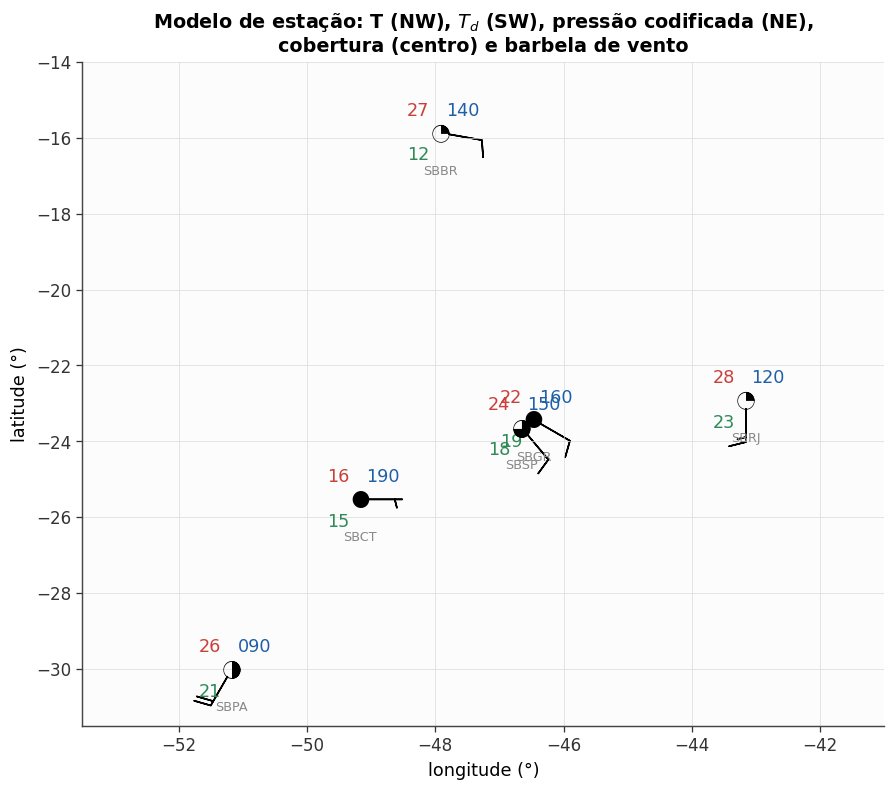
\includegraphics[width=\linewidth]{notebook_modelo_estacao.png}\\[-2pt]
    {\tiny modelo de estação com MetPy — Caso~2 do notebook do curso}\end{center}
  \end{columns}
\end{frame}

% ---------------------------------------------------------------
\section{Análise de cartas}

\begin{frame}{Redução ao nível do mar: sem ela não há carta}
  \eqdestaque{$P_{nm} = P_{est}\exp\!\left(\dfrac{g\,z_{est}}{\Re_d \bar
    T_v}\right)$}
  \vspace{0.5em}
  \begin{itemize}
    \item 10\,kPa a cada $\sim$840\,m: sem reduzir, o mapa de pressão é
          um mapa de \alert{altitude}.
    \item A hipsométrica do Cap.~1 em serviço operacional diário.
    \item Ponto fraco: a $\bar T_v$ de uma coluna que não existe —
          inversões enganam (T1).
    \item Antes × depois no Caso~4 do notebook.
  \end{itemize}
\end{frame}

\begin{frame}{Da nuvem de números ao campo}
  \begin{columns}
    \column{0.3\textwidth}
    \begin{itemize}
      \item Centenas de station plots $\to$ isóbaras a cada 4\,hPa.
      \item Fechar centros \textbf{A}/\textbf{B}; frentes nas dobras
            (Cap.~12).
      \item Aula prática: analisar esta carta a lápis.
    \end{itemize}
    \column{0.35\textwidth}
    \figlivroslide{fig_09_19.jpg}{0.46\textheight}{Fig.~9.19 --- as
      observações plotadas\ldots}
    \column{0.35\textwidth}
    \figlivroslide{fig_09_20.jpg}{0.46\textheight}{Fig.~9.20 --- \ldots e
      a análise pronta}
  \end{columns}
\end{frame}

\begin{frame}{Cartas reais: superfície e altitude}
  \begin{columns}
    \column{0.3\textwidth}
    \begin{itemize}
      \item Superfície: isóbaras $+$ frentes.
      \item 50\,kPa: alturas geopotenciais — colinas e vales cuja
            inclinação \alert{é} o vento (Cap.~10).
      \item Cavados de altitude comandam ciclones (Cap.~13).
    \end{itemize}
    \column{0.35\textwidth}
    \figlivroslide{fig_09_13a.jpg}{0.46\textheight}{Fig.~9.13 --- análise
      de pressão ao nível do mar}
    \column{0.35\textwidth}
    \figlivroslide{fig_09_13b.jpg}{0.46\textheight}{Fig.~9.13 --- alturas
      de 50\,kPa do mesmo instante}
  \end{columns}
\end{frame}

\begin{frame}{Regras de ouro da análise}
  \begin{columns}
    \column{0.55\textwidth}
    \begin{enumerate}
      \item Isóbaras a cada 4\,hPa, suaves, sem cruzar.
      \item Interpolar proporcionalmente entre estações.
      \item Fechar centros: \textbf{A} e \textbf{B}.
      \item Frentes nas dobras e contrastes (Cap.~12).
      \item Apertado $=$ ventoso (o porquê: Cap.~10).
    \end{enumerate}
    \vspace{0.4em}
    Em máquina: correções sucessivas (Cressman/Barnes) — o embrião da
    assimilação de dados (Cap.~20).
    \column{0.45\textwidth}
    \begin{center}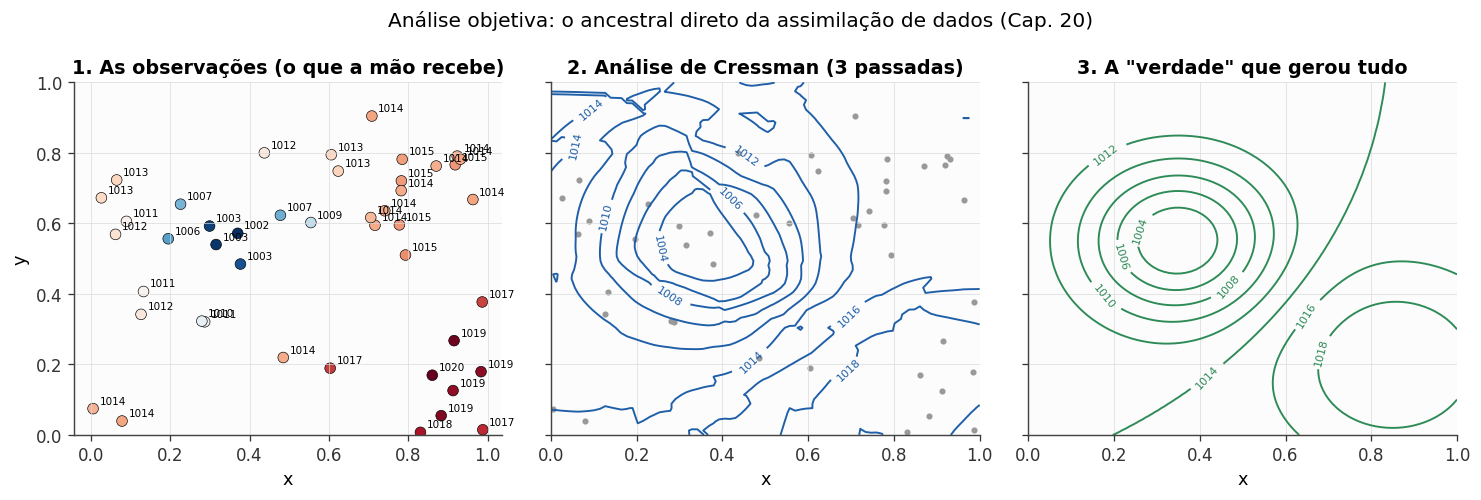
\includegraphics[width=\linewidth]{notebook_analise_objetiva.png}\\[-2pt]
    {\tiny análise objetiva de Cressman — Caso~3 do notebook do curso}\end{center}
  \end{columns}
\end{frame}

% ---------------------------------------------------------------
\section{Síntese e laboratório}

\begin{frame}{O mapa do capítulo}
  \eqdestaque{METAR $\to$ modelo de estação $\to$ redução ao nível do mar
    $\to$ isóbaras $\to$ Cap.~10}
  \vspace{0.6em}
  Alfabetização operacional: ler o código, plotar o ponto, desenhar o
  campo. A versão automática disso (análise objetiva) é o primeiro passo
  da previsão numérica.
\end{frame}

\begin{frame}{Laboratório numérico --- notebook do Cap.~9}
  \texttt{notebooks/cap09\_cartas.ipynb}
  \begin{enumerate}
    \item Parser de METAR em Python (aeroportos brasileiros).
    \item Modelo de estação com o MetPy.
    \item Análise objetiva de Cressman: de pontos a isóbaras.
    \item Redução ao nível do mar: o mapa errado × o mapa sinótico.
  \end{enumerate}
  \vspace{0.4em}
  \textbf{Exercícios}: T1--T5 e N1--N4 nas notas; células reservadas no
  notebook. Aula prática sugerida: análise manual de carta impressa do
  dia.
  \vfill
  \atribuicao
\end{frame}

\end{document}
